\chapter[Revisão Sistemática]{Revisão Sistemática}

    Este capítulo apresenta conceitos pertinentes aos principais tópicos que serão abordados
    nesse TCC. Os tópicos abordados são, \textit{Hadoop, MapReduce, Spark, Impala, HBase e
    Cloudera.}

    \section{Hadoop}

            O \textit{Hadoop} foi criado por Doug Cutting, o mesmo criador do Apache Lucene, a biblioteca de busca
            textual \cite{white2015}. O \textit{Hadoop} é composto por dois componentes principais, o HDFS que é
            um sistema de arquivos para ser usado em \textit{cluster}, e o \textit{MapReduce} que é responsável
            pelo processamento dos dados armazenados no sistema de arquivos. O \textit{Hadoop} em comparação
            com outros sistemas de arquivos distribuídos possui é um sistema tolerante a falhas críticas, e foi
            desenvolvido para rodar em máquinas de baixo custo com um modelo de programação simples
            \cite{alam2014}. Segundo \citeonline{alam2014}, o \textit{Hadoop} cobre quase todos os aspectos dos
            paradigmas de sistemas distribuídos como confiabilidade, eficiência, disponibilidade, acurácia e segurança.

        \subsection{Hadoop Distributed File System}

            O HDFS é um sistema de arquivos distribuídos desenvolvido para armazenar arquivos muito grandes
            com um padrão de fluxo de dados, que funcionam dentro de um \textit{cluster} de máquinas de baixo
            custo \cite{white2015}.

            As suas principais características são, lotes de grandes arquivos a serem processados, o fluxo de acesso
            de dados em que o sistema escreve uma vez e lê várias vezes em determinado padrão e pôr fim a baixa
            necessidade de uma estrutura de ponta, pois o próprio sistema já fornece quase todos os aspectos dos
            paradigmas que os sistemas distribuídos tentam cobrir, logo foi desenvolvido para rodar em máquinas de
            baixo custo (computadores domésticos são exemplos de máquinas de baixo custo), o sistema se utiliza de
            implementações contra falhas críticas para, caso um \textit{node} venha a falhar o HDFS ainda continue
            trabalhando sem interrupções \cite{white2015}.

            \subsubsection{Bloco de Dados}

                O conceito de bloco de dados, se refere ao \textit{container} que será utilizado para o armazenamento
                dos dados. Este \textit{container} possui um tamanho padrão que pode ser definido nas configurações
                do HDFS dependendo da necessidade do cliente. O bloco de dados então é armazenado ao longo do
                \textit{cluster} e suas referências são guardadas.

                O motivo pelo qual se dá preferência a arquivos muito grandes, é pela necessidade de dividir esses
                arquivos em blocos, para que encaixem nos \textit{containers}. Para \citeonline{white2015}, ter
                uma abstração de bloco para um \textit{Distributed Filesystem} (DFS) pode trazer uma série de
                benefícios como o caso de um arquivo ser maior que o disco, então existe a vantagem de ter vários
                discos em \textit{cluster}.

                Outra vantagem, está na abstração dos blocos ao invés de arquivos, e isso simplifica o armazenamento.
                O subsistema de armazenamento usa blocos de dados para simplificar o gerenciamento de armazenamento,
                pois como os blocos possuem tamanhos fixos, fica fácil determinar a alocação dos blocos ao longo dos
                discos \cite{white2015}.

                Não existe necessidade de preocupação com os metadados levando em consideração que os blocos são
                apenas pedaços de dados que são armazenados, já os arquivos de metadados tais como informações sobre
                permissões não precisam ser armazenados com os blocos, pois existe outro sistema que trata dos metadados
                separadamente \cite{shvachko2010}.

                \begin{figure}[ht!]
                    \centering
                    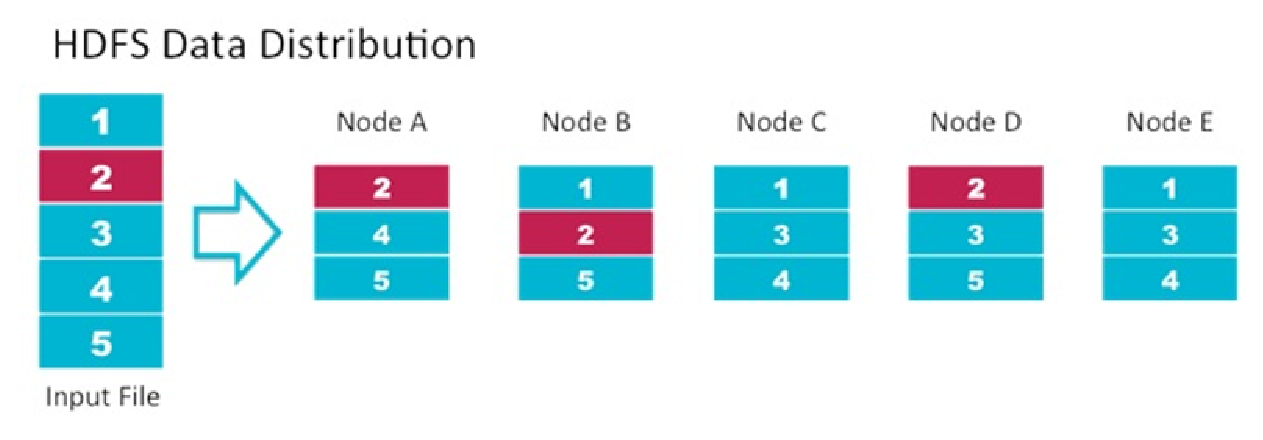
\includegraphics[keepaspectratio=true,scale=0.75]
                        {figuras/figura1.eps}
                    \caption[Distribuição em Blocos no HDFS]{Distribuição em Blocos no HDFS
                    \protect\linebreak Fonte: \citeonline{hadoopexample}}
                    \label{figura1}
                \end{figure}

                Com a replicação dos dados, temos a garantia de que mesmo que um \textit{node} venha a falhar o dado
                não será perdido, garantindo a proteção contra falhas críticas e disponibilidade. Essa replicação é realizada
                por padrão de distribuição em até três maquinas, mas essa configuração pode ser alterada dependendo da
                necessidade do cliente para garantir a integridade de seus dados.

            \subsubsection{Arquitetura HDFS}

                Em um cluster de HDFS, existem dois tipos de \textit{nodes} operantes no caso o: \textit{namenode} (\textit{master})
                e um certo número de \textit{datanodes} (trabalhadores). O \textit{namenode} gerencia o \textit{namespace} e
                mantêm a arvore do sistema de arquivos e dos metadados para todos os arquivos e diretórios na estrutura. Essa
                informação é armazenada no disco local em forma de dois arquivos, a imagem do \textit{namespace} e o log de edição.
                De acordo com \citeonline{shvachko2010}, o \textit{namenode} conhece em quais \textit{datanodes}  determinado
                arquivo está localizado, porém ele não reconstrói o local, por que essa informação é reconstruída a partir dos
                \textit{datanodes} quando o sistema inicia \cite{white2015}.

                O \textit{client} acessa o sistema de arquivos em nome do usuário, se comunicando com o \textit{namenode} e
                \textit{datanodes}. A interface do \textit{client} é similar ao \textit{Portable Operating System Interface} (sistema
                que o kernel do Linux usa), logo o usuário não precisa saber sobre as funções do \textit{namenode} e
                \textit{datanodes} em específico.

                \begin{figure}[ht!]
                    \centering
                    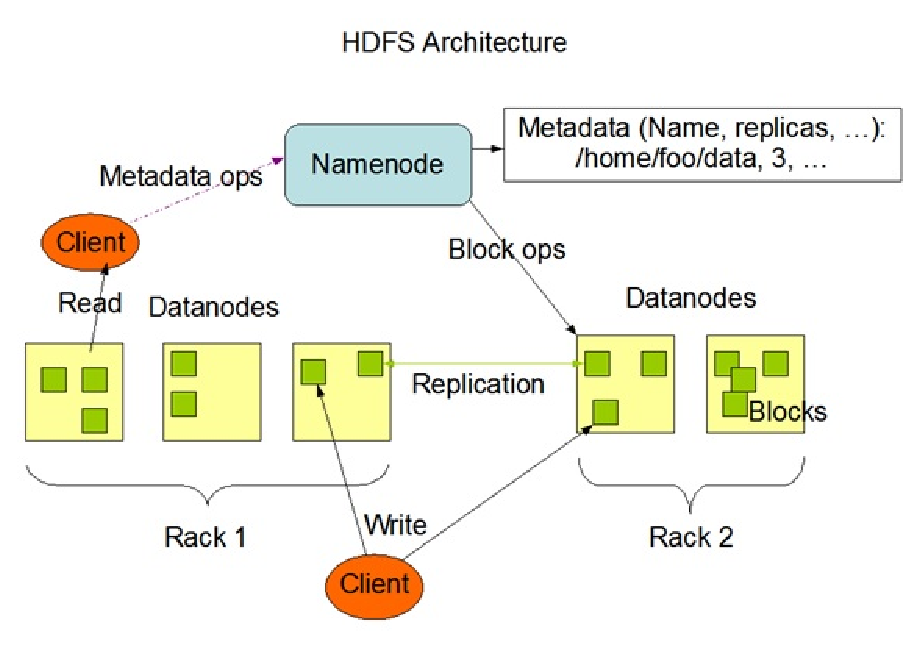
\includegraphics[keepaspectratio=true,scale=0.75]
                        {figuras/figura2.eps}
                    \caption[Arquitetura do HDFS]{Arquitetura do HDFS
                    \protect\linebreak Fonte: \citeonline{hadoopapache}}
                    \label{figura2}
                \end{figure}

                Na figura \ref{figura2}, temos a visualização da arquitetura do HDFS, o \textit{namenode} manipula
                os metadados que são essenciais para a aplicação \textit{client}, nele temos dados do \textit{namespace}
                e o número de réplicas bem como outras informações a mais, e com o mapeamento desses dados a aplicação
                consegue recuperar o dado que precisa nos \textit{datanodes} referenciados.

            \subsubsection{Processo de Leitura e Escrita}

                Quando uma aplicação vai ler um arquivo, o HDFS \textit{client} pergunta ao \textit{namenode} pela lista
                de \textit{datanodes} que guardam as réplicas de determinado bloco do arquivo. Só então a aplicação
                comunica-se com o \textit{datanode} diretamente e requisita a transferência de determinado bloco. É
                possível visualizar esse processo de forma detalhada na figura 3, o qual temos uma aplicação do HDFS
                em cima de uma \textit{Java Virtual Machine} (JVM) que se comunica com os \textit{nodes} em determinada
                ordem, para obter um determinado arquivo \cite{shvachko2010}.

                Já quando a aplicação escreve, ele pergunta ao \textit{namenode} para que escolha os \textit{datanodes}
                que serão utilizado para armazenar o primeiro bloco do arquivo, então o \textit{client} organiza uma
                \textit{pipeline} de \textit{node} para \textit{node} e envia os dados. Quando o primeiro bloco é preenchido,
                o \textit{client} faz uma nova requisição por novos \textit{datanodes} a serem escolhidos para guardarem
                as réplicas do próximo bloco. Esse mesmo processo é possível de ser visualizado na figura 4 com detalhes
                \cite{shvachko2010}.

                \begin{figure}[ht!]
                    \centering
                    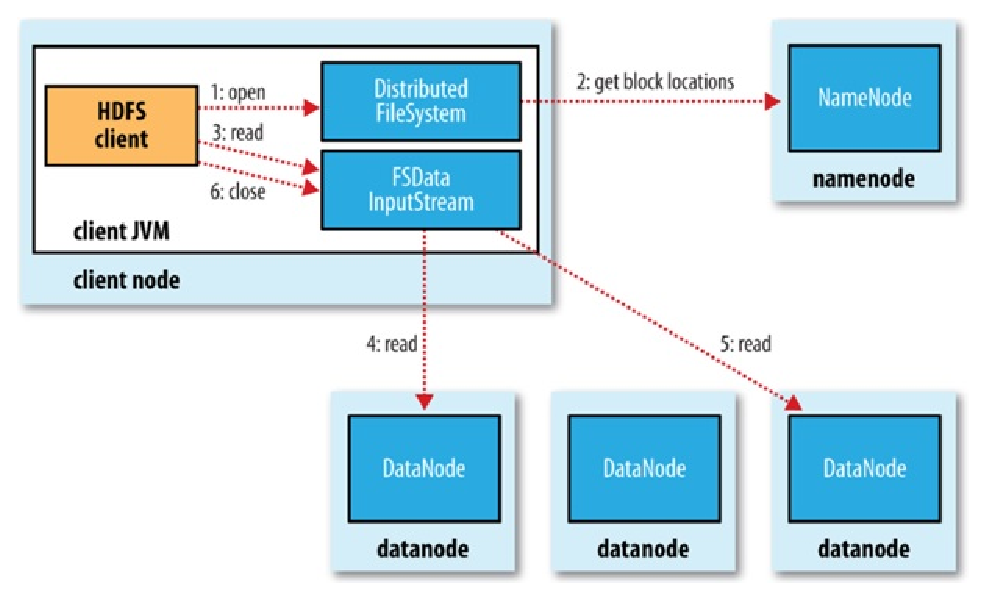
\includegraphics[keepaspectratio=true,scale=0.75]
                        {figuras/figura3.eps}
                    \caption[Processo de Leitura no HDFS]{Processo de Leitura no HDFS
                    \protect\linebreak Fonte: \citeonline{white2015}}
                    \label{figura3}
                \end{figure}

                \begin{figure}[ht!]
                    \centering
                    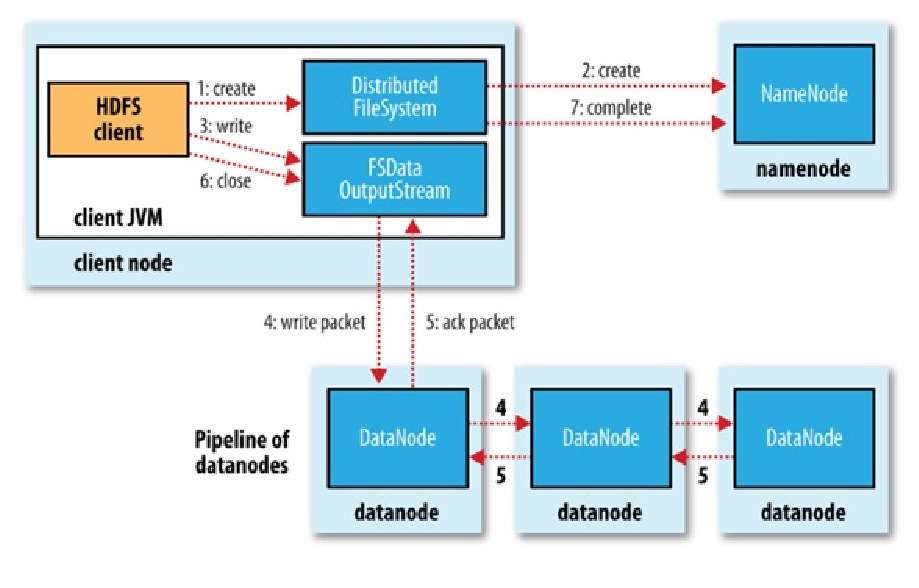
\includegraphics[keepaspectratio=true,scale=0.75]
                        {figuras/figura4.eps}
                    \caption[Processo de Escrita no HDFS]{Processo de Escrita no HDFS
                    \protect\linebreak Fonte: \citeonline{white2015}}
                    \label{figura4}
                \end{figure}

        \subsection{MapReduce}

            O desenvolvimento do \textit{MapReduce} surgiu de uma necessidade de processamento de uma grande
            quantidade de dados brutos, com o objetivo  de computar diversos tipos de dados derivados, como índices,
            representações gráficas acerca de determinados dados, sumarização, dentre outras \textit{queries} frequentes
            usadas no dia-a-dia. Porém os dados de entrada são geralmente grandes e computacionalmente precisam ser
            distribuídos ao longo de milhares de máquinas, para que seja possível de terminar em uma quantidade de
            tempo razoável \cite{dean2008}.

            De acordo com \citeonline{dean2008}, o \textit{MapReduce} foi desenvolvido em resposta a complexidade
            que se tem para processamento de dados em lote em uma arquitetura distribuída. Então essa camada de
            abstração permite expressar uma computação mais simples, mas que por baixo, abstrai detalhes de computação
            paralela, tolerância a falhas, distribuição de dados e balanceamento de carga só que em uma biblioteca.

            O \textit{MapReduce} funciona quebrando o processo em duas fases, a fase de \textit{map} e a fase de
            \textit{reduce}. Cada fase tem um par de \{chave,valor\} como entrada e saída. O programador também
            especifica as duas funções, a função de \textit{map} e a função de \textit{reduce} \cite{white2015}.

            A função \textit{map} escrita pelo usuário, precisa de um par na entrada e produz um intervalo de pares de
            \{chave,valor\}. A biblioteca agrupa juntamente com todos os valores intermediários associados com a mesma
            chave intermediária e repassa para a função \textit{reduce}. Já a função \textit{reduce} aceita uma chave
            intermediária e um intervalor de valores para aquela chave. Esses valores são agrupados para forma um
            intervalo menor ainda de valores, tipicamente apenas zeros ou uma entrada de valores produzidos por
            invocação do \textit{reduce}. Esses valores intermediários são produzidos pelas funções \textit{reduce}
            do usuário que vão sendo iteradas. Isto nos permite manejar a lista de valores que são muito grandes
            para caber na memória \cite{dean2008}.

            De acordo com \citeonline{white2015} o \textit{MapReduce job} é uma unidade de trabalho que a
            aplicação deseja que seja processada, e consiste em uma entrada de dados, a definição do
            \textit{MapReduce} programado e a configuração das informações. O Hadoop executa o \textit{job}
            dividindo ele em dois tipos de tarefas, as chamadas \textit{map tasks} e \textit{reduce tasks}.
            Essas tarefas são organizadas usando o YARN (\textit{Yet Another Resource Negotiator}) e são
            executadas nos \textit{nodes} do cluster, e se a tarefa falha, ela será automaticamente reorganizada
            para a fila de execução em um \textit{node} diferente. Na figura \ref{figura5} temos a ilustração no
            processo \textit{shuffle} e \textit{sort}  que é um processo que garante que toda entrada para cada
            \textit{reduce} tenha uma chave, e que valor seja repassado a saída do \textit{map} para as
            entradas das funções \textit{reduce}\cite{white2015}.

            \begin{figure}[ht!]
                    \centering
                    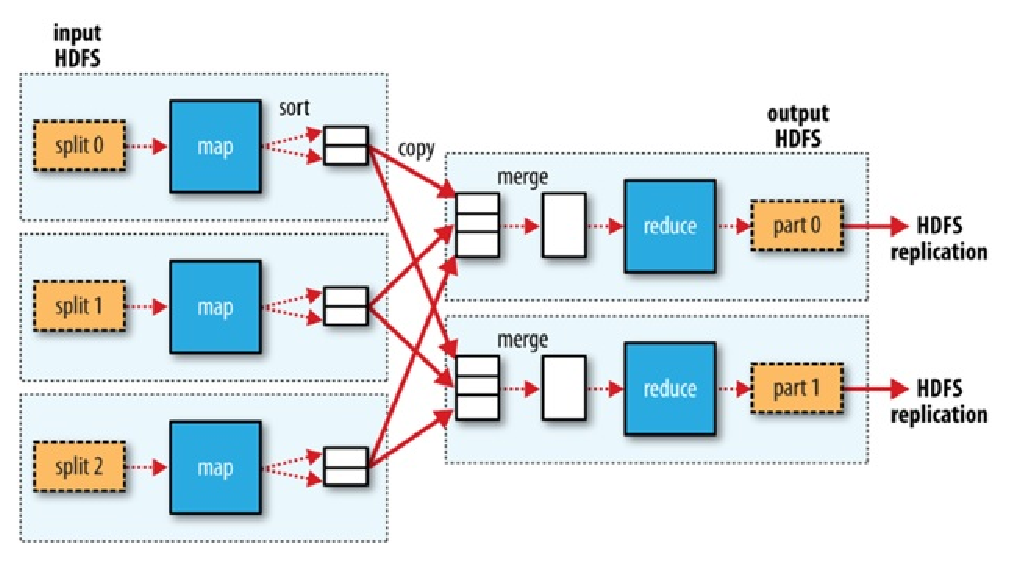
\includegraphics[keepaspectratio=true,scale=0.75]
                        {figuras/figura5.eps}
                    \caption[Fluxo de dados em um \textit{MapReduce} com múltiplas tarefas de redução]
                    {Fluxo de dados em um \textit{MapReduce} com múltiplas tarefas de redução
                    \protect \linebreak Fonte: \citeonline{white2015}}
                    \label{figura5}
            \end{figure}

            \subsubsection{Arquitetura do MapReduce}

                Para entendermos a arquitetura do \textit{MapReduce}, vamos passar por algumas fases do processo.
                O \textit{Hadoop} divide a entrada de dados dos \textit{MapReduce jobs} em pedaços de tamanho fixo
                chamados \textit{input splits}. O \textit{Hadoop} então cria um \textit{map task} para cada cada \textit{split},
                e roda as configurações definidas pelo usuário na função \textit{map} para cada registro do \textit{split}.
                Com vários \textit{splits} significa que o tempo de processamento de cada \textit{split} é menor
                comparado ao tempo de processamento de um \textit{split} completo. Se estamos processando os
                \textit{splits} em paralelo, o balanceamento de carga é mais efetivo, já quando os \textit{splits} são
                pequenos, uma máquina rápida irá processar mais \textit{splits} comparado a uma máquina lenta
                \cite{white2015}.

                A invocação do \textit{map} é distribuída, ao longo de várias máquinas automaticamente particionando
                os dados de entrada em intervalor de vários \textit{splits}. Os \textit{input splits} podem ser processados
                em paralelo em diferentes máquinas. As invocações do \textit{reducer} são distribuídas pelo
                particionamento do espaço da chave intermediária em vários \textit{splits} usando a função de
                particionamento. O número de partições e de funções de particionamento são especificadas pelo usuário.

                Na figura \ref{figura6} abaixo temos a visualização do fluxo geral das operações do \textit{MapReduce}.
                Quando um programa chama as funções de \textit{MapReduce}, a seguinte sequência de ações ocorre.
                A biblioteca do \textit{MapReduce} no programa do usuário divide os arquivos de entrada em vários
                \textit{splits} tipicamente de 64-128MB por \textit{split}. Então ele inicia várias instancias do programa
                no \textit{cluster} indicado \cite{dean2008}.

                De acordo com \citeonline{dean2008}, uma das instancias do programa (o \textit{master}) é especial.
                O resto são trabalhadores que terão tarefas designadas pelo \textit{master}. Existem vários \textit{map tasks}
                e  \textit{reduce tasks} a serem atribuídos. O \textit{master} decide os trabalhadores, que estão ociosos,
                para atribuir a cada um deles um \textit{map task} e um \textit{reduce task} que serão processados. O
                trabalhador que foi atribuído ao \textit{map task} irá ler o conteúdo do \textit{input split} correspondente.
                Ele analisa o par de \{chave,valor\} dos dados de entrada e repassa cada par a função de \textit{map}
                definida pelo usuário. Os pares de {chave,valor} intermediários serão produzidos pela função de \textit{map}
                que está armazenada em \textit{buffer} na memória.

                Tanto para \citeonline{dean2008} quanto para \citeonline{white2015}, ambos explicam que periodicamente,
                os pares que estão em \textit{buffer} são escritos no disco local, e particionados em regiões pela função de
                particionamento. A localização desses pares em \textit{buffer} no disco local é repassada ao \textit{master}
                que irá se responsabilizar pelo repasse dessas localizações aos \textit{reduce workers}. Quando um \textit{
                reduce worker} é notificado pelo \textit{master} sobre a localização, ele usa um recursos chamado \textit{
                Remote Procedure Calls} (RPC) para ler os dados do \textit{buffer} do disco local dos \textit{map workers}.
                Então depois que o \textit{reduce worker} lê todos os dados intermediários da partição, ele organiza por
                chave intermediária para que todas as ocorrências da mesma chave sejam agrupadas. A organização é
                necessária por causa que diferentes chaves são mapeadas para o mesmo \textit{reduce task}. E se esse
                agrupamento de dados intermediários for muito grande para caber em memória, uma organização externa
                será necessária.

                O \textit{reduce worker} itera sobre os dados intermediários organizados e para cada chave intermediária
                única encontrada, ele repassa a chave e o intervalo de valores intermediários correspondentes a função de
                \textit{reduce} do usuário. A saída da função \textit{reduce} é acrescentada ao final do arquivo de saída
                para essa partição do \textit{reduce}. Quando todos os \textit{map tasks} e \textit{reduce tasks} forem
                completados, o \textit{master} acorda a aplicação. Nesse ponto o \textit{MapReduce} repassa o retorno
                da aplicação para o código do usuário \cite{dean2008}.

                \begin{figure}[ht!]
                    \centering
                    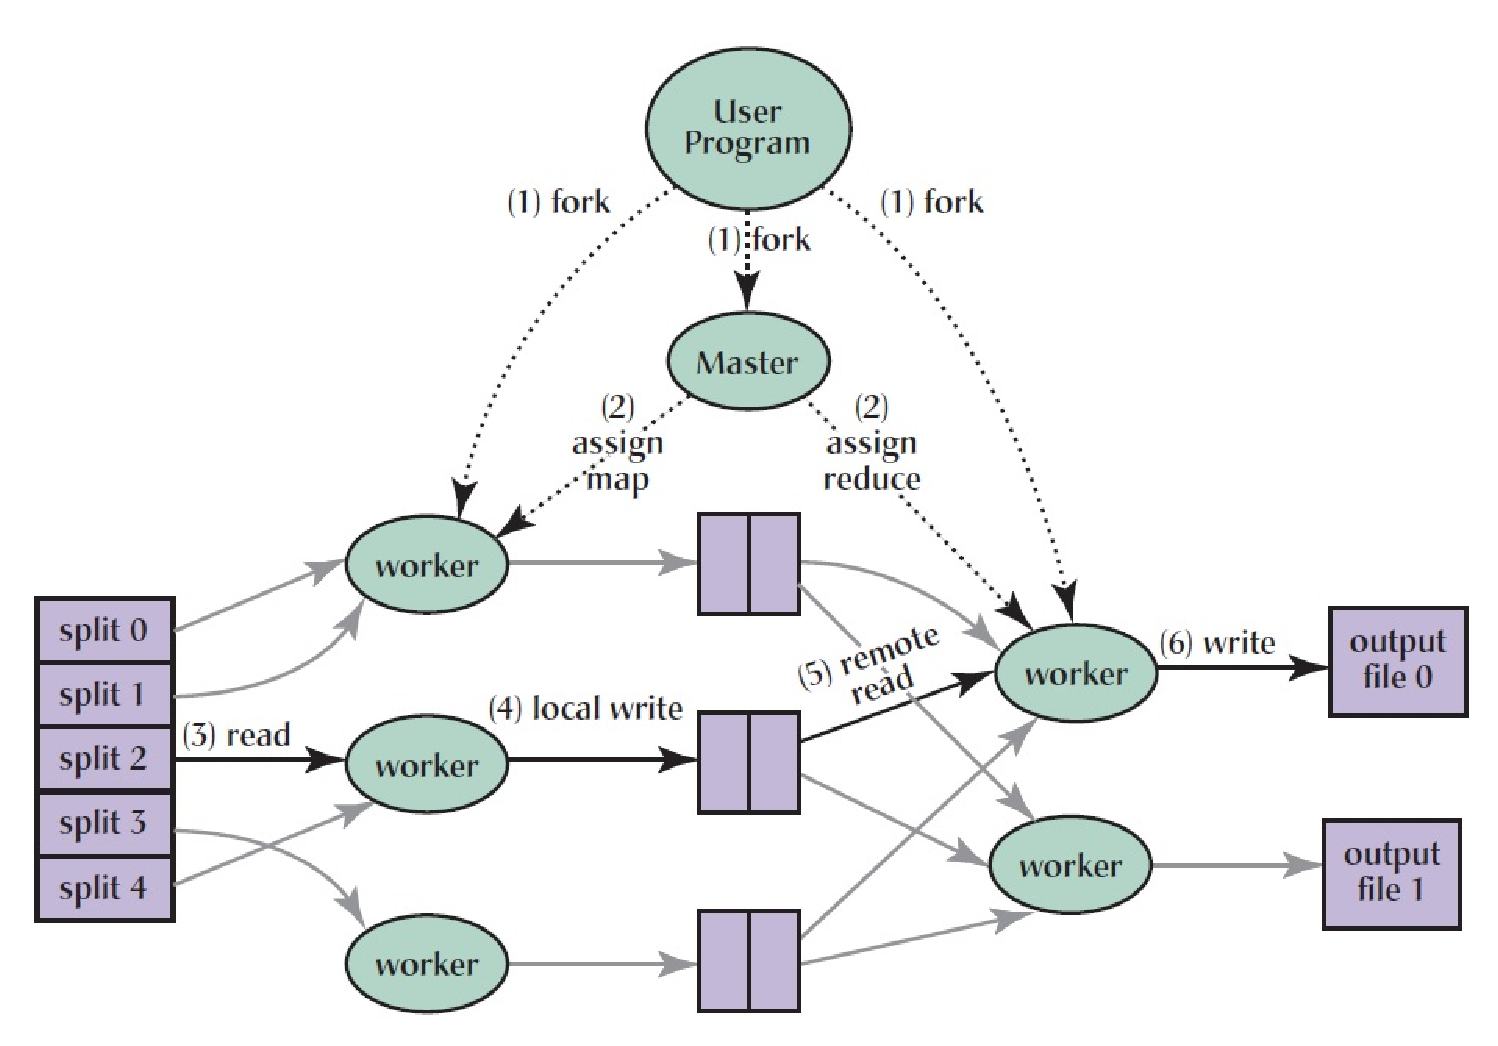
\includegraphics[keepaspectratio=true,scale=0.5]
                        {figuras/figura6.eps}
                    \caption[Fluxo de dados do processo de execução do \textit{MapReduce}]
                    {Fluxo de dados do processo de execução do \textit{MapReduce}
                    \protect \linebreak Fonte: \citeonline{dean2008}}
                    \label{figura6}
                \end{figure}

        \subsection{YARN}

            Apache YARN (\textit{Yet Another Resource Negotiator}) é um sistema de gerenciamento de recursos para
            um \textit{cluster Hadoop}. O YARN foi introduzido nas novas versões do \textit{Hadoop} 2.x para melhorar
            a implementação do \textit{MapReduce}, mas em geral é usado para suporta outros paradigmas da
            computação distribuída também \cite{yarnapache}.

            Segundo as explicações de \citeonline{vavilapalli2013}, o YARN provê dois tipos de serviços essenciais que são
            executados em \textit{background}, o \textit{resource manager} para gerenciamento do uso de recursos ao
            longo do \textit{cluster}, e os \textit{node managers} que são executados em todos os \textit{nodes} de um
            \textit{cluster}, para monitorar os \textit{containers}. O \textit{container} executa um processo de aplicação
            específica com restrição a uma série de recursos (memória, CPU e etc.).

            \begin{figure}[ht!]
                        \centering
                        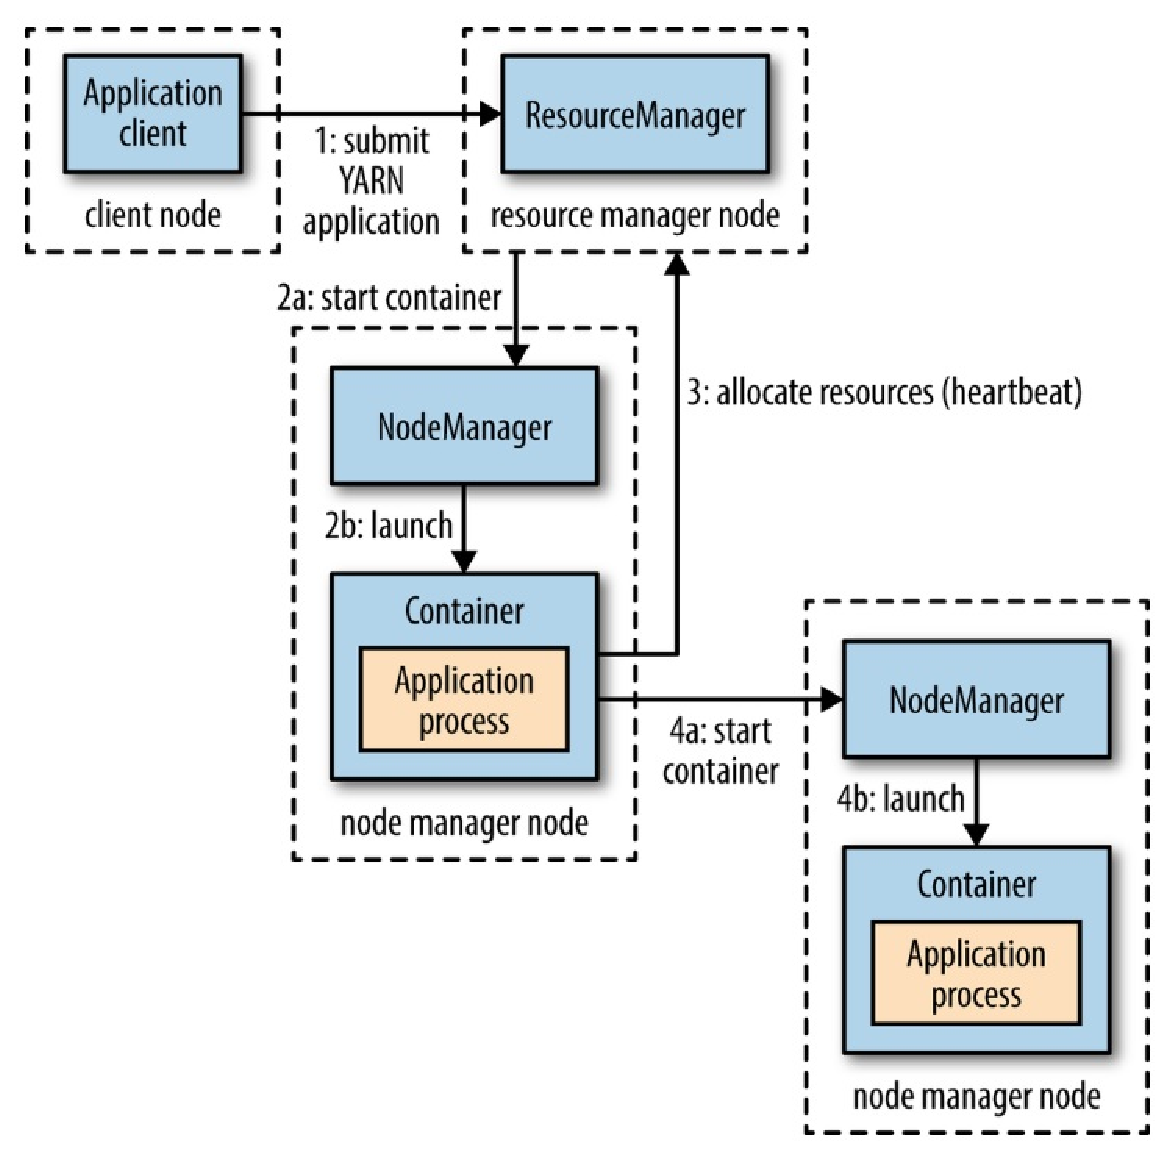
\includegraphics[keepaspectratio=true,scale=0.5]
                            {figuras/figura7.eps}
                        \caption[Anatomia de um processo em execução no YARN]{Anatomia de um processo em execução no YARN
                        \protect \linebreak Fonte: \citeonline{white2015}}
                        \label{figura7}
            \end{figure}

            Para executar uma aplicação no YARN, o \textit{client} chama o \textit{resource manager} e pede para executar
            o \textit{application master process}. O \textit{resource manager} então procura um \textit{node manager} que
            possa executar o \textit{application master} em um \textit{container}. A execução do \textit{application master}
            vai depender do comportamento da aplicação \cite{vavilapalli2013}. Na figura \ref{figura7} temos a arquitetura de
            execução de um \textit{application master} no YARN, então vários passos são executados até chegar a melhor
            otimização possível de recursos em paralelo com as outros \textit{jobs} em execução.

            \subsubsection{Requisição de Recursos}

                O YARN possui um modelo de flexibilidade para realização de requisição de recursos. Uma requisição para um
                intervalor de \textit{containers} pode ser expressa por um percentual dos recursos computacionais requeridos
                para cada container, bem como as restrições de localidades para cada \textit{container} naquela determinada
                requisição \cite{white2015}.

                A localidade é crítica em garantir que o algoritmo de processamento de dados distribuídos use a banda do
                \textit{cluster} de forma eficiente, então o YARN permite que a aplicação especifique as restrições de
                localidade para as requisições dos \textit{containers} \cite{vavilapalli2013}. Requisições de localidade
                podem ser usadas para requisitar um \textit{container} em um \textit{node, rack} ou qualquer outro lugar
                especifico fora do \textit{rack} \cite{white2015}.

            \subsubsection{Tempo de Vida da Aplicação}

                O tempo de vida de uma aplicação YARN pode variar bastante de um pequeno ciclo de apenas alguns segundos
                a um grande ciclo que possui um tempo de execução de dias ou meses. A eficiência de um tempo de vida da
                aplicação recai na categorização das aplicações em termos de como realizar o mapeamento dos \textit{jobs}
                que o usuário executa \cite{yarnapache}.

                O caso mais simples é a de uma aplicação do \textit{job} de usuário, que é a mesma aproximação utilizadas pelas
                \textit{tasks} do \textit{MapReduce}. O segundo modelo é a de rodar uma aplicação por fluxo ou por sessão de
                usuário. Essa aproximação pode ser mais eficiente que a primeira, já que os \textit{containers} podem ser reusados
                entre os \textit{jobs}, e ainda existe o potencial de \textit{cache} intermediário entre os \textit{jobs}
                \cite{yarnapache}.

            \subsubsection{Tipos de Agendamento}

                O objetivo do YARN está como um gerenciador de recursos que irá realocar os recursos para as aplicações de acordo
                com uma política definida. Agendamento em geral é um problema complexo, e não existe uma política ideal, por isso
                que o YARN disponibiliza escolhas para gerenciamento do agendamento de recursos e configurações das políticas de
                agendamento \cite{vavilapalli2013}.

                O \citeonline{white2015} elabora sobre o YARN, explicando que ele disponibiliza três tipos de agendamento de recursos,
                que são o \textit{First In First Out} (FIFO), \textit{Capacity} e o \textit{Fair Schedulers}. O agendamento usando FIFO
                organiza as aplicações em uma fila por ordem de submissão em que o primeiro a entrar é o primeiro a sair. Requisições
                para a primeira aplicação, que para \citeonline{white2015}, são alocadas primeiramente na fila, depois que as requisições
                forem satisfeitas, a próxima aplicação é executada e assim por diante.

                De acordo com \citeonline{white2015} e com a complementação de \citeonline{vavilapalli2013}, ambos relatam que para o
                agendamento \textit{Capacity}, uma fila dedicada é criada separadamente que irá permitir que pequenos \textit{jobs}
                iniciem assim que possível após terem sido submetidos, só que esse tipo de configuração possui um custo de utilização
                da capacidade do \textit{cluster} quase todo já que a capacidade da fila é reservada para \textit{jobs} que estão
                naquela fila. Isso significa que \textit{jobs} maiores irão terminar mais tarde, com essa determinada configuração.

                O \textit{Fair Scheduler} é uma configuração em que não existe a necessidade de reservar um percentual da
                capacidade, desde que os recursos sejam dinamicamente balanceados entre os \textit{jobs} que estão sendo executados.
                Só depois que um \textit{job} grande for executado, que esse será o único \textit{job} executado no momento, então ele
                terá acesso a todos os recursos no cluster. Quando um \textit{job} pequeno inicia, os recursos do cluster serão alocados de
                forma justa, e assim por diante de acordo com o tamanho do \textit{job}, logo cada \textit{job} terá de dividir os recursos de
                forma justa para os outros \textit{jobs} que estão sendo executados simultaneamente \cite{white2015}.

                \begin{figure}[ht!]
                        \centering
                        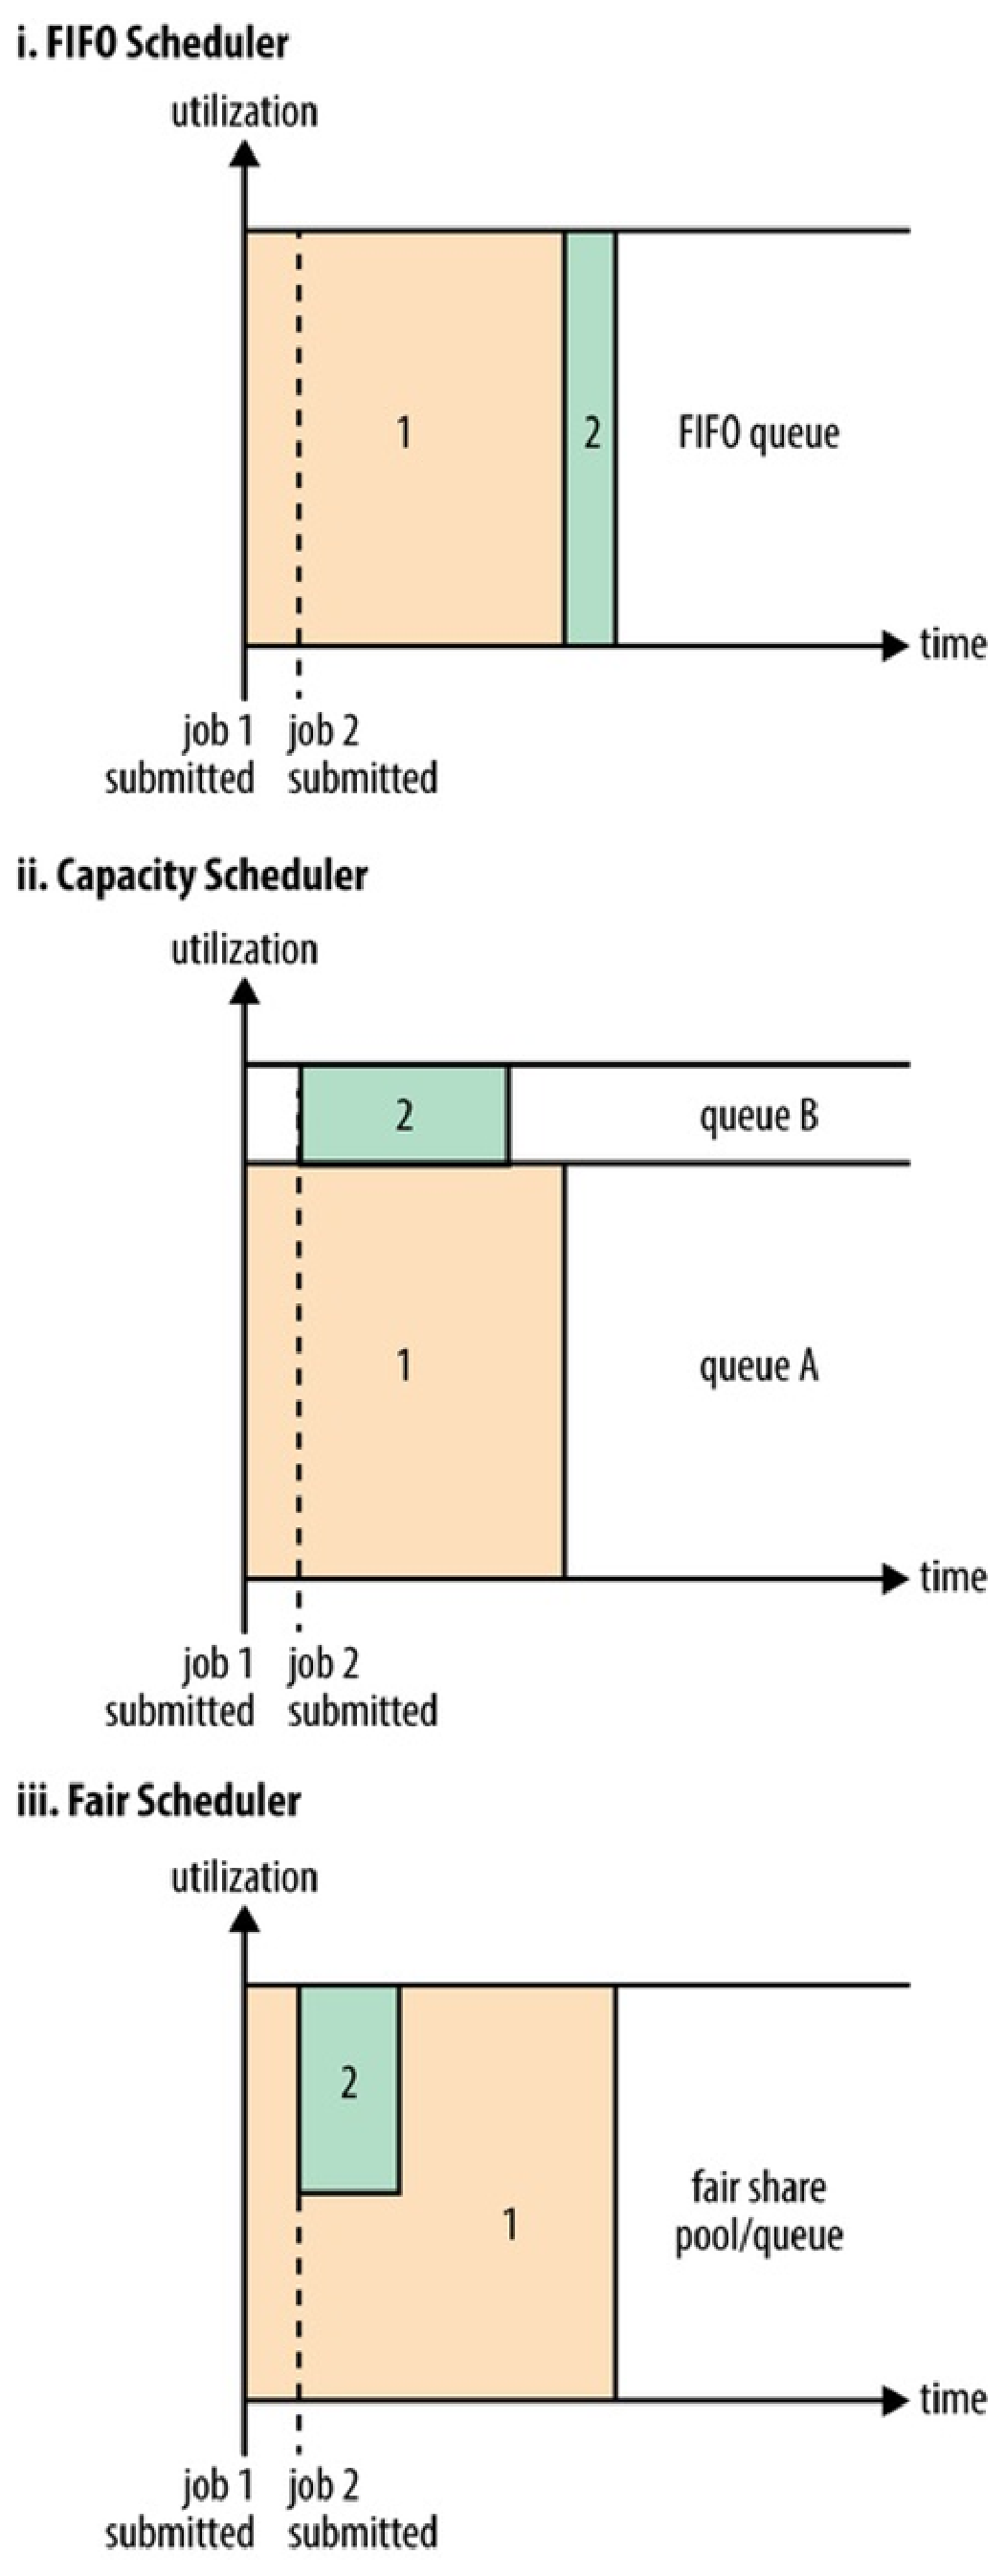
\includegraphics[keepaspectratio=true,scale=0.30]
                            {figuras/figura8.eps}
                        \caption[Opções de agendamento do YARN]{Opções de agendamento do YARN
                        \protect \linebreak Fonte: \citeonline{white2015}}
                        \label{figura8}
                 \end{figure}

    \section{HBase}

        Os bancos de dados de hoje em dia se preocupam em realizar transações. Vivemos uma atualidade, o qual a profissão de
        Administrador de Banco de dados acaba se tornando um cargo de bastante importância nas organizações. O responsável
        pelo banco de dados irá ser responsável por manter os dados da organização e persisti-los de modo que não haja nenhum
        problema, isso junto ao ACID (\textit{Atomic, Consistency, Isolation, Durability}) pois os bancos de dados relacionais são
        baseados no modelo transacional. Agora em relação aos projetos em que não exista essa preocupação grande com os
        dados, e exista um grande volume de dados, grandes corporações acabam adotando um modelo não convencional,
        que é baseado em uma solução com um banco de dados não relacional.

        O autor do livro \textit{HBase: The definitive guide} por \citeonline{george2011} explica que o \textit{HBase} é um
        banco de dados distribuídos orientado a coluna construído em cima do HDFS. Ele aprofunda sua explicação relatando
        que o \textit{HBase} é uma aplicação \textit{Hadoop} para ser usada quando existe a necessidade de leitura e escrita
        randômica em tempo real para modelos de dados gigantes (\textit{datasets} de bilhões de colunas por milhões de linhas).
        O \textit{HBase} escala o problema por uma perspectiva diferente, ele foi construído utilizando uma abordagem
        \textit{down-top} com escalabilidade linear, ou seja, apenas adicionando novos \textit{nodes} ao \textit{cluster}.

        \subsection{NoSQL}

            Os bancos de dados não relacionais, que são NoSQL (\textit{Not only Structured Query Language}), são ferramentas
            que vão de auxílio para ajudar no gerenciamento de dados interno, de uma forma mais simples em relação a um
            banco de dados relacional. Segundo \citeonline{moniruzzaman2013} o movimento pela adoção dessa tecnologia
            tem mudado os horizontes de comportamento dos dados. O principal ponto que o autor defende é referente a
            tecnologia tanto de bancos relacionais quanto não-relacionais de poderem coexistir e possuírem seu espaço
            guardado no mercado. Empresas como Facebook, Twitter, Amazon, LinkedIn e Google, utilizam banco de dados
            NoSQL de uma forma ou outra, para tratar seus grandes volumes de dados na área de Big Data com o auxílio do
            grande ecossistema de ferramentas como Apache \textit{Hadoop}, dentre outras \cite{moniruzzaman2013}.

            Os autores \citeonline{strauch2011} e \citeonline{moniruzzaman2013} demonstram que, a integridade de dados
            é garantida pela maioria dos bancos de dados atuais que são baseados no modelo transacional, pois isso garante
            a consistência dos dados em situações referentes ao gerenciamento desses dados. De acordo
            \citeonline{moniruzzaman2013} existe um teorema chamado CAP (\textit{Consistancy, Availability, Partition Tolerance})
            que trata das características previstas nos bancos de dados não relacionais. Na figura \ref{figura9} apresenta uma
            relação entre esses principais conceitos.

            Este diagrama segundo o autor \citeonline{moniruzzaman2013} explica os seguintes atributos: \textit{Consistancy}
            (Consistência) que trata sobre todos os clientes que acessam os dados atuais independente de atualizações e
            remoções de dados. O atributo \textit{Availability} (Disponibilidade) que aborda a necessidade dos sistemas de
            continuarem operando como esperado, mesmo em caso de um \textit{node} falhar. Por último temos o \textit{Partition
            Tolerance} (Tolerância a partição) que trata da continuidade de operação do sistema como esperado, mesmo que a rede,
            ou a troca de mensagens entre os \textit{nodes} venham a falhar.

            \begin{figure}[ht!]
                        \centering
                        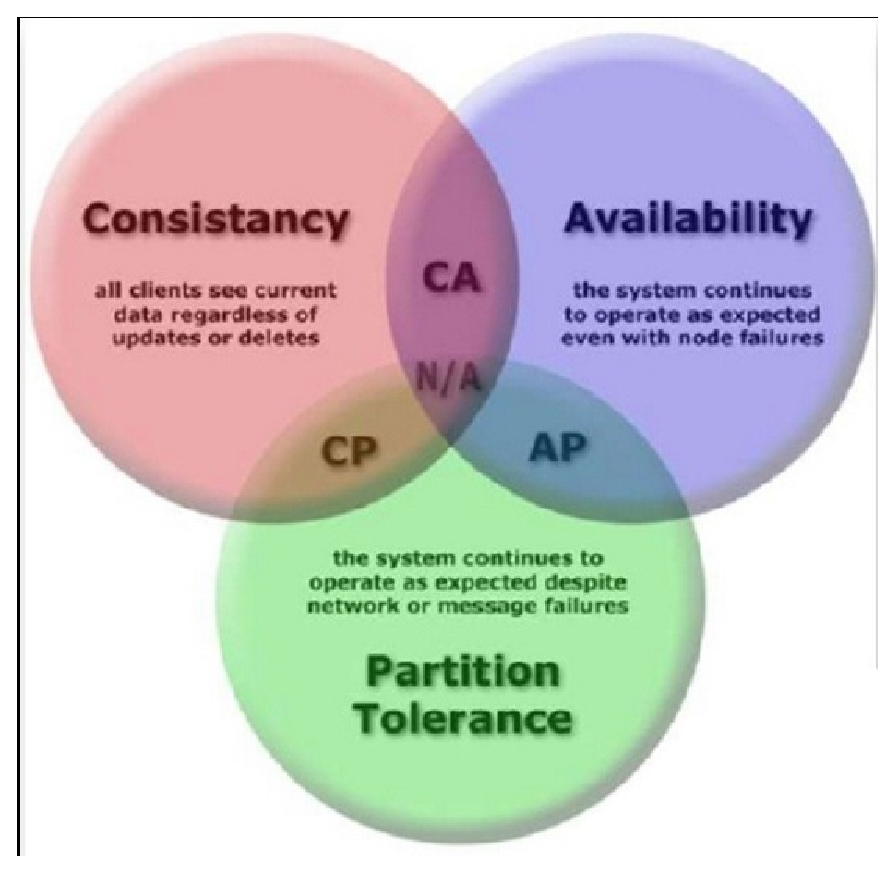
\includegraphics[keepaspectratio=true,scale=0.5]
                            {figuras/figura9.eps}
                        \caption[Características do NoSQL]{Características do NoSQL
                        \protect \linebreak Fonte: \citeonline{moniruzzaman2013}}
                        \label{figura9}
            \end{figure}

            Com a implantação do teorema CAP, o ACID não atenderia muito bem as expectativas do NoSQL, para isso surgiu o
            BASE seguido das seguintes características:  \textit{Basically Available, Soft-state, Eventual consistency} que trata
            sobre características referentes as operações do NoSQL. É possível fazer uma analogia de como se fosse \textit{Design
            Patterns} para Bancos de dados distribuídos não relacionais. Dentre as características do BASE podemos citar a fraca
            consistência de dados, disponibilidade em primeiro lugar, melhor eficiência, aproximação de respostas, simples, rápido
            e evolucionário \cite{moniruzzaman2013}.

        \subsection{Modelagem de Dados}

            O \textit{HBase} é um banco de dados não relacional, ou seja, ele não suporta SQL. Ele foi baseado no \textit{Google’s
            Bigtable}, e foi evoluído em um projeto \textit{open source} no fim de 2006 e teve sua primeira release lançada junto ao
            \textit{Hadoop} em Outubro de 2007 \cite{white2015}.

            Aprofundando a arquitetura do \textit{HBase}, \citeonline{vora2011} explica que a aplicação armazena dados em
            tabelas que foram determinadas. Essas tabelas são feitas de linhas e colunas. Cada tabela-célula é uma intersecção
            coordenada entre uma linha e coluna, e todas elas são versionadas. Por padrão, o versionamento é um \textit{timestamp}
            colocado automaticamente pelo \textit{HBase} e ele ocorre no momento da inserção de dados na célula. O conteúdo da
            célula é um \textit{Byte Array} não interpretado. Na figura \ref{figura10} abaixo pode-se visualizar o esquema do modelo
            de dados que é rearranjado no \textit{HBase}.

            \begin{figure}[ht!]
                        \centering
                        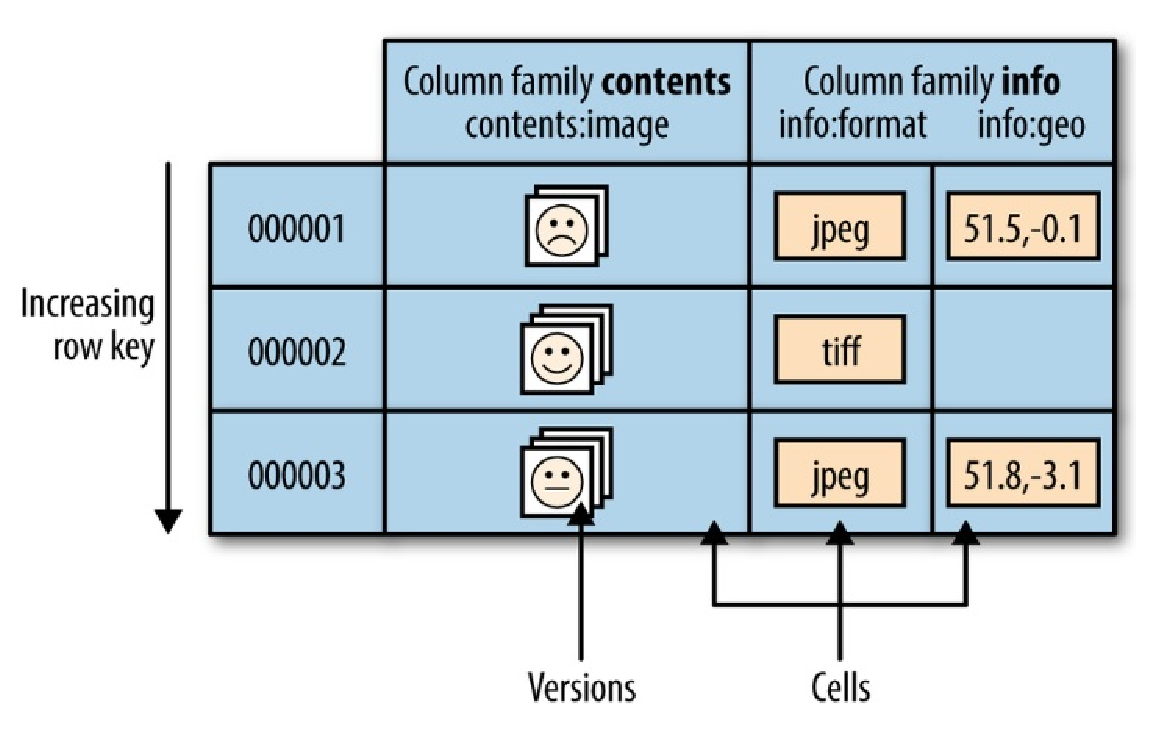
\includegraphics[keepaspectratio=true,scale=0.5]
                            {figuras/figura10.eps}
                        \caption[Estrutura do Modelo de Dados no HBase]{Estrutura do Modelo de Dados no HBase -
                        \protect Fonte: \citeonline{white2015}}
                        \label{figura10}
            \end{figure}

            O esquema organizacional do \textit{HBase} se baseia no conceito de coluna família, que são agrupamentos de colunas
            de linhas. Todos os membros da coluna família têm um prefixo em comum, então por exemplo, na figura \ref{figura10}
            temos uma coluna família chamada \textit{info} e nela temos colunas de linhas uma chamada \textit{format} e a outra
            chamada \textit{geo}, que são reconhecidas pelo comando \textit{info:format} e \textit{info:geo}, pois remetem a coluna
            família \textit{info} e as colunas de linhas chamadas \textit{format} e \textit{geo} para aquela coluna família em específico
            \cite{white2015}.

        \subsection{Arquitetura}

            Explicação de \citeonline{george2011} apresenta que as tabelas do \textit{HBase} são automaticamente particionadas
            horizontalmente pelo \textit{cluster} em \textit{regions} (regiões). Cada \textit{region} (região) contém um intervalo
            de linhas de uma tabela. Inicialmente a tabela tenta comprimir os dados para que fiquem apenas em uma \textit{region},
            mas ao longo do crescimento dos dados na tabela, a \textit{region} vai alcançando seu limite até que eventualmente
            acabe sendo necessário particionar os dados de uma tabela em mais de uma \textit{region}. \textit{Regions} são
            unidades que são distribuídas ao longo de um \textit{cluster HBase}. Neste quesito, se uma tabela é grande demais
            para um servidor, ela será distribuída ao longo dos \textit{nodes} do \textit{cluster}, com cada \textit{node} guardando
            um intervalo de \textit{regions} total da tabela em específico.

            A estrutura do \textit{HBase} é organizada em um \textit{master node} que organiza o \textit{cluster} em vários
            \textit{regionserver workers} \cite{carstoiu2010}. Segundo o artigo de \citeonline{carstoiu2010}, o \textit{HBase
            master} possui a responsabilidade de organizar os \textit{regions} para os \textit{regionservers} registrados e por
            recuperar as falhas do \textit{regionserver}. O \textit{master node} pode ficar um pouco sobrecarregado enquanto
            que os \textit{regionservers} carregam \textit{regions} e requisições de leitura e escrita. Eles também gerenciam
            \textit{region splits}, informando ao \textit{master node} sobre as novas \textit{regions} filhas para que ele possa
            gerenciar os \textit{regions} parentes, bem como a possibilidade de atribuir substituições para as filhas ao longo do
            gerenciamento de \textit{regions}. Referente a figura \ref{figura11} temos a ilustração da arquitetura do \textit{HBase}
            em um \textit{cluster}, com o seus \textit{nodes} específicos, e na figura \ref{figura12} é ilustrado a arquitetura e o
            comportamento do \textit{regionserver}.

            O \textit{HBase} possui uma dependência com \textit{ZooKeeper}, pois essa é uma ferramenta de gerenciamento
            de serviços distribuídos, e o \textit{HBase} controla as instâncias do \textit{ZooKeeper} para manter o controle no
            cluster \cite{george2011}.  O \textit{ZooKeeper} possui um papel vital, ele possui a localização dos metadados do
            \textit{HBase}, bem como as informações das tabelas e o endereço do \textit{cluster master} atual. A atribuição de
            \textit{regions} é mediada pelo \textit{ZooKeeper} em caso dos servidores participantes caírem no meio da atribuição.
            O \textit{ZooKeeper} também serve como um controle de serviços que o \textit{cluster} tem a oferecer, com isso
            centralizando todos os serviços em um só lugar \cite{vora2011}. Na tabela \ref{tabela1} temos a ilustração das
            principais características que o \textit{HBase} fornece para as organizações e projetos que forem usá-los.

            \begin{figure}[ht!]
                        \centering
                        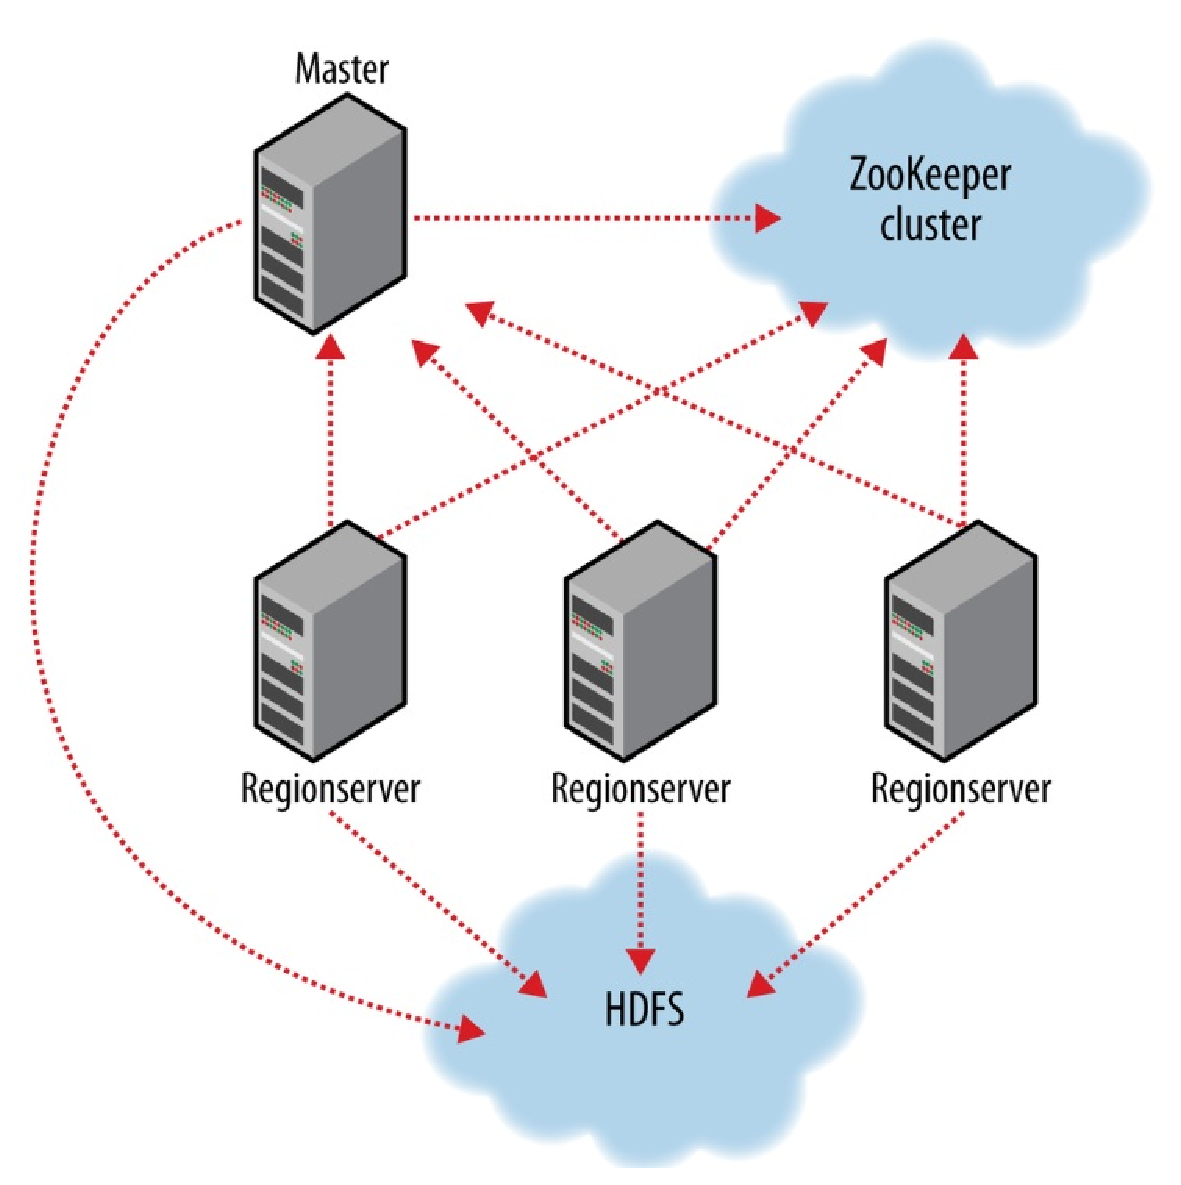
\includegraphics[keepaspectratio=true,scale=0.5]
                            {figuras/figura11.eps}
                        \caption[Arquitetura de um \textit{cluster} HBase]{Arquitetura de um \textit{cluster} HBase
                        \protect \linebreak Fonte: \citeonline{white2015}}
                        \label{figura11}
            \end{figure}

            \begin{figure}[ht!]
                        \centering
                        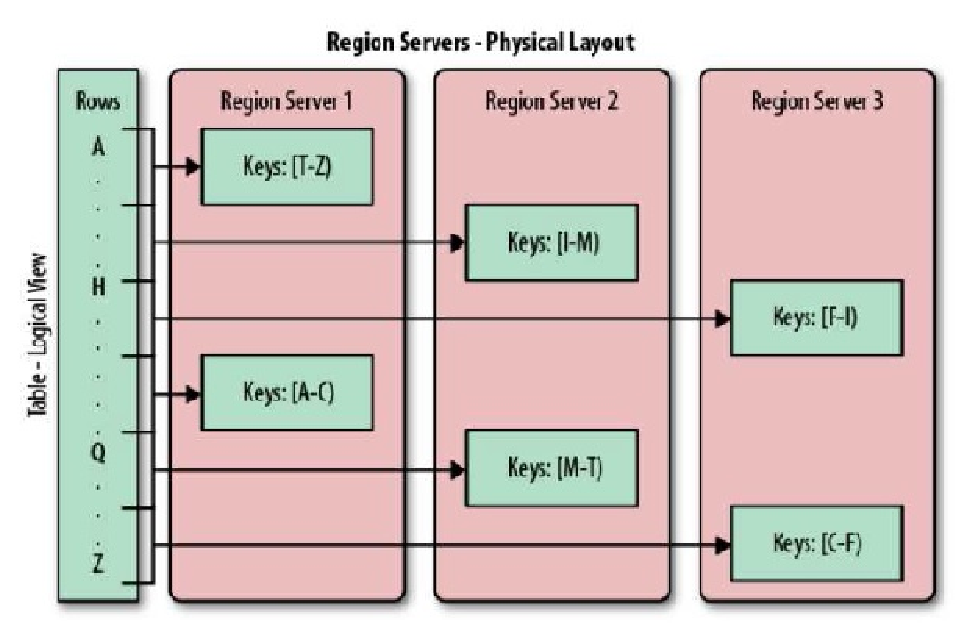
\includegraphics[keepaspectratio=true,scale=0.7]
                            {figuras/figura12.eps}
                        \caption[\textit{Regionserver} no HBase]{\textit{Regionserver} no HBase -
                        \protect Fonte: \citeonline{george2011}}
                        \label{figura12}
            \end{figure}

            \begin{table}[!ht]
            \begin{center}
              \begin{tabular}{|p{8cm}|p{8cm}|}
                \hline
                Caracteristicas do HBase & Descrição
                \\ \hline
                Não possui indexação & As linhas são armazenadas sequencialmente,
                                                        assim como as colunas em cada linha. Não existe
                                                        sobrecarga de indexação, e o desempenho da
                                                        inserção é independente do tamanho da tabela.
                \\ \hline
                Particionamento automático & Conforme as tabelas vão crescendo, elas vão sendo divididas em
                                                                    \textit{regions} e distribuídas ao longo dos \textit{nodes}.
                \\ \hline
                Escalabilidade linear e automática com novos nodes & Possibilidade de adição de novos \textit{nodes} para um
                                                                                                          determinado \textit{cluster}, e execução de \textit{regionserver}
                                                                                                          nesses novos \textit{nodes}. Os \textit{regions} serão
                                                                                                          automaticamente balanceados e carregados igualmente ao longo
                                                                                                          dos novos \textit{regionserver}.
                \\ \hline
                Hardware barato para suporta o \textit{HBase} & Não existe necessidade de um hardware de alta capacidade
                                                                                                  para executar essa ferramenta.
                \\ \hline
                Tolerância a falhas & Vários \textit{nodes} significa que cada um é relativamente insignificante. Não existe
                                                    necessidade de se preocupar com a falha de um \textit{node} individual.
                \\ \hline
                Processamento em Lote & Integração com \textit{MapReduce} permite paralelizar totalmente,
                                                            distribuir \textit{jobs} com relacionado aos dados com o conhecimento da localidade.
                \\ \hline
              \end{tabular}
              \caption[Características do HBase]{Características do HBase -
              \protect Fonte: Adaptado de \citeonline{white2015} e \citeonline{george2011}}
            \label{tabela1}
            \end{center}
            \end{table}

    \section{Spark}

        Neste capítulo será explicado o conceito da ferramenta \textit{Spark}. Uma ferramenta de processamento que auxilia o
        \textit{MapReduce} e se integra junto a outras ferramentas. Essa ferramenta produzida em 2009 na universidade de
        \textit{Berkeley} nos Estados Unidos, a ferramenta ganhou um apoio muito forte da comunidade Apache o qual mantem
        a ferramenta bem como suporte do Cloudera. Essa ferramenta veio para trazer um conceito evolutivo nas atividades de
        processamento em \textit{Big Data}.

        Apache \textit{Spark} é uma plataforma de processamento em cluster designada para ser rápida e possuir um propósito
        de processamento genérico \cite{karau2015}. O Spark oferece um suporte eficiente ao modelo \textit{MapReduce} para
        diferentes tipos processamento computacional, incluindo \textit{queries} interativas e \textit{stream processing}.
        Velocidade é importante em relação ao processamento de grandes \textit{datasets}, e isso significa diferença entre
        explorar os dados interativamente ou esperar minutos ou horas. Uma das principais características do \textit{Spark} é a
        habilidade de executar processamento em memória, e esse sistema é mais eficiente que o \textit{MapReduce} para
        aplicações complexas executadas em disco \cite{karau2015}.

        O auto \citeonline{karau2015} explica que o \textit{Spark} foi desenvolvido para executar um processamento extensivo que
        antigamente era requerida com sistemas distribuídos separados, incluído aplicações em lote, algoritmos iterativos, \textit{queries}
        interativas e \textit{streaming}. Por suporta esse tipo de processamento com a mesma \textit{engine}, o \textit{Spark}
        tornou fácil e não tão caro a combinação de diferentes tipos de processamento, que são necessários na produção da
        análise de dados em \textit{pipeline}. Em complemento pode-se dizer que ele reduz a carga de gerenciamento e da manutenção
        de ferramentas em especifico \cite{karau2015}.

        Segundo \citeonline{white2015}, o \textit{Spark} foi desenvolvido para ser altamente acessível, oferecendo API’s simples
        em Python, Java, Scala e SQL, além de ser construído em um rico acervo de bibliotecas. Ele também se integra com outras
        ferramentas de \textit{Big Data}, em particular o \textit{Spark} pode ser executado junto aos \textit{clusters} de
        \textit{Hadoop} sem contar de poder acessar o HDFS, incluindo \textit{HBase}.

        Uma das características principais do Spark que \citeonline{white2015} explica, é a capacidade dele trabalhar com um
        grande acervo de \textit{datasets} em memória. Essa capacidade permite o \textit{Spark} trabalhar com uma eficiência
        maior que o fluxo de trabalho do \textit{MapReduce}, ao qual os \textit{datasets} são sempre carregados do disco.

        \subsection{Módulos do Spark}

            O \textit{Spark} é composto por uma série de módulos que integradas permitem que a aplicação possa trabalhar em
            diversos campos de processamento de dados no \textit{Big Data} \cite{karau2015}. Desde algoritmos iterativos que
            permitem que uma função seja aplicada várias vezes ao \textit{dataset} até que a condição de saída aconteça, bem
            como analises interativas que permitem ao usuário executar uma série de \textit{queries} exploratórias no \textit{dataset},
            ao invés de ficar esperando pelo resultado \cite{white2015}. A figura \ref{figura13} ilustra os módulos do \textit{Spark},
            bem como as ferramentas de gerenciamento de \textit{clusters} ao qual ele se integra.

            \begin{figure}[ht!]
                        \centering
                        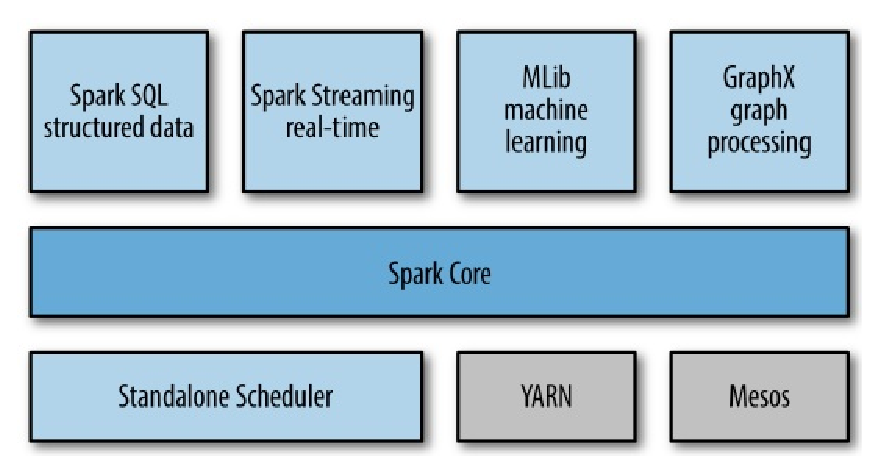
\includegraphics[keepaspectratio=true,scale=0.7]
                            {figuras/figura13.eps}
                        \caption[Módulos do Spark]{Módulos do Spark
                        \protect \linebreak Fonte: \citeonline{karau2015}}
                        \label{figura13}
            \end{figure}

            Seguindo ao que o diagrama da figura \ref{figura13} temos o \textit{core} do Spark, que contém funcionalidades
            básicas ao \textit{Spark}, que incluem componentes para agendamento de \textit{tasks}, gerenciamento de
            memória, recuperação de falhas, interação com os sistemas de armazenamento e mais. O \textit{core} também
            fornece \textit{API’s} que definem o chamado \textit{Resilient Distributed Datasets} (RDDs) que são as principais
            bibliotecas de abstração da programação do \textit{Spark} \cite{karau2015}.

            O módulo de \textit{Spark} SQL fornece um pacote que trabalha com dados estruturados. Ele permite realizar
            \textit{queries} via SQL bem como pelo Apache \textit{Hive} variante do SQL chamada \textit{Hive Query Language}
            (HQL). Ele suporta várias fontes de dados, incluindo tabelas \textit{Hive, Parquet} e JSON. Além de fornecer uma
            interface SQL ao \textit{Spark}, este módulo permite que os desenvolvedores misturem \textit{queries} SQL com
            manipulações de dados via programação, suportada pelos RDDs de Python, Java e Scala, tudo isso em uma só aplicação,
            combinando SQL a uma complexidade analítica \cite{karau2015}.

            Referente ao módulo de \textit{Spark Streaming}, este componente permite processamento de \textit{stream} de dados
            ao vivo. Este módulo fornece uma API para manipulação de \textit{stream} de dados que é semelhante ao \textit{core}
            do \textit{Spark} referente as API’s dos RDD’s, tornando mais fácil para os programadores aprenderem o projeto e permitir
            mover entre aplicações que manipulam dados armazenados em memória, no disco, ou que chegam em tempo real. Debaixo
            dessa API, este módulo foi desenvolvido para fornecer o mesmo nível de tolerância a falha, taxa de transferência e
            escalabilidade assim como o \textit{core} do \textit{Spark} \cite{karau2015}.

            Um módulo bastante interessante no que se referente ao quesito de aprendizagem de máquina, o \textit{Spark} tem um
            módulo que contém bibliotecas para funcionalidades de \textit{Machine Learning} chamadas MLlib. Esse módulo fornece
            múltiplos tipos de algoritmos para \textit{machine learning}, incluindo classificação, regressão, \textit{clustering}, e filtros
            colaborativos, bem como funcionalidades de suporte a modelos e importação de dados \cite{karau2015}.

            Outro módulo que faz parte do \textit{Spark} é o \textit{GraphX}, uma biblioteca para manipulação de grafos, e para
            realização de processamento em paralelo de grafos. Como o \textit{Spark Streaming} e \textit{Spark} SQL, o \textit{GraphX}
            estende do \textit{Spark} RDD API, que permite criar grafos diretamente com propriedades arbitrárias em anexo para cada
            vértice e ponta. \textit{GraphX} também fornece várias operações de manipulação de grafos e uma biblioteca com os algoritmos
            de grafos mais comuns \cite{karau2015}.

            De baixo da camada de abstração do Spark, foi desenvolvido um sistema para alcançar uma eficiência alta em escala de
            um \textit{node} para vários \textit{nodes} computacionais. Com o objetivo de alcançar a máxima flexibilidade, o Spark
            pode executar uma variedade de gerentes de cluster, incluindo \textit{Hadoop} YARN, Apache \textit{Mesos} e um simples
            gerente de cluster incluído no próprio \textit{Spark}, chamado \textit{Standalone Scheduler} \cite{karau2015}.

        \subsection{Resilient Distributed Datasets}

            As abstrações realizadas no \textit{Spark}, são feitas com base nas RDDs que é o coração do Spark. As RDDs são abstrações
            que dão ao usuário o controle do compartilhamento de dados. Essas RDDs também são tolerantes a falha, possuem estrutura
            de dados paralelas que permitem ao usuário armazenar dados em disco ou na memória explicitamente, as RDDs também
            controlam o particionamento, e manipulam usando um grande acervo de operadores. Eles oferecem uma maneira simples
            e uma interface de programação eficiente que captura tanto os modelos especializados quanto novas aplicações
            \cite{zaharia2013}.

            Na definição de \citeonline{zaharia2013}, uma RDD é apenas para leitura, particionada em uma coleção de registros.
            As RDDs podem ser criadas apenas por operações determinísticas em um dado no armazenamento estável ou por outras
            RDDs. Essas operações são chamadas de \textit{transformations} para diferencia-las de outras operações no RDDs.
            Exemplo dessas operações de transformação incluem \textit{map, filter} e \textit{join} \cite{karau2015}.

            Os usuários podem controlar outros aspectos dos RDDs, no caso \textit{persistence} e \textit{partitioning}. Os usuários
            também podem indicar os RDDs que serão reusados e escolher o armazenamento estratégico para eles. Outra ação que
            pode ser realizada é pedir que os elementos do RDD sejam particionados ao longo do \textit{cluster} utilizando uma
            chave para cada registro, e esta ação fornece uma otimização que garante a possibilidade de juntar dois \textit{datasets}
            que são particionados usando uma única \textit{hash} que garante o controle das partições \cite{zaharia2013}.

             \begin{figure}[ht!]
                        \centering
                        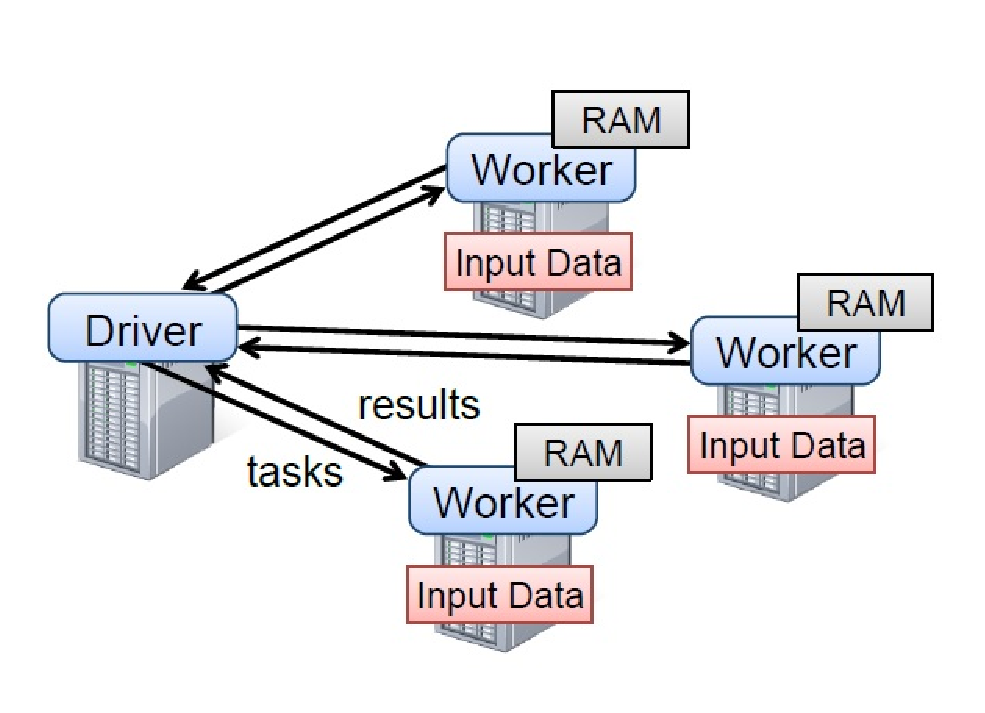
\includegraphics[keepaspectratio=true,scale=0.5]
                            {figuras/figura14.eps}
                        \caption[Execução no Spark]{Execução no Spark
                        \protect \linebreak Fonte: \citeonline{zaharia2013}}
                        \label{figura14}
            \end{figure}

        \subsection{Representação dos RDDs}

            O autor \citeonline{zaharia2013} que foi um dos responsáveis por surgir com o conceito de representação dos RDDs
            relata que um dos desafios em fornecer RDDs como abstração era escolher a representação para eles, e como seria
            possível rastrear o \textit{lineage} (Um log sobre as transformações realizadas em determinado RDD) ao longo de
            um intervalo de transformações. Idealmente, a implementação do sistema de RDDs deveria fornecer um uma série
            operadores de transformações, para dar um poder de escolha aos usuários em elaborar suas próprias ações de forma
            arbitrária. A resolução deste problema se baseou na representação do RDD na forma de um grafo, pois essa representação
            suporta uma série de transformações sem a necessidade de adicionar alguma lógica especial ao agendamento de cada RDD,
            o que simplificou bastante o design do sistema \cite{zaharia2013}.

            A camada de interface do RDD, oferece acesso a informações essenciais como: o intervalo de \textit{dependencies}
            que são pedaços atômicos do \textit{dataset}, uma série de \textit{dependencies} nos RDDs pais, uma função para
            computar o \textit{dataset} baseado nos pais, e os metadados sobre o esquema de particionamento bem como a
            localização dos dados \cite{karau2015}.

            As dependências dos RDDs são classificadas em dois tipos: \textit{narrow dependencies} que define cada partição do RDD
            pai que é usada pelo menos em uma partição do RDD filho, e temos o \textit{wide dependencies} quando tem-se múltiplas
            partições filhas que dependem dessa \textit{dependencie} \cite{karau2015}.

            A explicação de \citeonline{zaharia2013} apresenta dois motivos para necessidade dessa distinção: o primeiro relata que
            as \textit{narrow dependencies} permitem a execução de uma pipeline em um \textit{node} do \textit{cluster}, o qual
            pode computar todos as partições dos pais. Em contraste, \textit{wide dependencies} requerem dados de todas as partições
            dos pais que estejam disponíveis para que sejam distribuídas ao longo dos \textit{nodes} usando a operação parecida com a
            do MapReduce. Segundo, diz em relação a recuperação após a falha de um \textit{node} ser mais eficiente com
            \textit{narrow dependency}, já que apenas uma partição parente precisa ser reprocessada e ela pode ser processada novamente
            em paralelo em diferentes \textit{nodes}. Em contraste, um grafo de \textit{lineage} com \textit{wide dependencies}, caso tenha
            uma única falha no \textit{node}, isso pode causar a perda de algumas partições de todos os ancestrais de um RDD, assim
            criando a necessidade de processar novamente por completo.

            \begin{table}[!ht]
            \begin{center}
              \begin{tabular}{|p{5cm}|p{10cm}|}
                \hline
                Transformação & Descrição
                \\ \hline
                HDFS \textit{files} & A entrada nos RDDs são amostra de arquivos no HDFS.  Para esses RDDs, partições retornam
                                                   uma partição para cada bloco de arquivo, \textit{preferredLocations} da aos \textit{nodes}
                                                   que o bloco está pronto, e que o \textit{iterator} está pronto para ler o bloco.
                \\ \hline
                \textit{map} & Chamando \textit{map} em qualquer RDD, retorna um objeto \textit{MappedRDD}. Esse objeto tem
                                          as mesmas partições e localizações favoritas que seus pais, mas aplica a função para \textit{map}
                                          para os registros dos pais em um método \textit{iterator}.
                \\ \hline
                \textit{union} & Chamando \textit{union} em duas RDDs retorna uma RDD cuja as partições é a união dos pais.
                                            Cada partição filha é computada por uma \textit{narrow dependency} em um pai.
                \\ \hline
                \textit{sample} & Amostragem é similar ao mapeamento, exceto que o RDD armazena um gerador de número
                                              aleatório para cada partição com o objetivo de determinar a amostragem dos registros do pai.
                \\ \hline
                \textit{join} & Juntando duas RDDs pode levar a duas \textit{narrow dependencies}, ou a duas \textit{wide dependencies},
                                        ou uma mistura. Em ambos os casos, a saída é um RDD com um ou vários particionamentos.
                \\ \hline
              \end{tabular}
              \caption[Transformações comuns no RDD]{Transformações comuns no RDD -
              \protect Fonte: Adaptado de \citeonline{zaharia2013} e \citeonline{karau2015}}
            \label{tabela2}
            \end{center}
            \end{table}

            \begin{table}[!ht]
            \begin{center}
              \begin{tabular}{|p{5cm}|p{8cm}|}
                \hline
                Operação & Significado
                \\ \hline
                \textit{partitions()} & Retorna uma lista de objetos de \textit{Partition}.
                \\ \hline
                \textit{preferredLocations(p)} & Lista os \textit{nodes} aonde a partição p pode ser acessada rapidamente
                                                                     devido a localidade do dado.
                \\ \hline
                \textit{dependencies()} & Retorna lista de \textit{dependencies}.
                \\ \hline
                \textit{iterator(p, parentIters)} & Processa os elementos da partição p dados os \textit{iterators} para
                                                                       as partições do pai.
                \\ \hline
                \textit{partitioner()} & Retorna os metadados específicos quando o RDD é particionado num intervalo \textit{hash}.
                \\ \hline
              \end{tabular}
              \caption[Interface utilizada para representar os RDDs no Spark]{Interface utilizada para representar os RDDs no Spark -
              \protect Fonte: \citeonline{zaharia2013}}
            \label{tabela3}
            \end{center}
            \end{table}

        \subsection{Implementação e Agendamento de Jobs}

            O \textit{Spark} se integra com a entrada de dados do \textit{Hadoop} (HDFS ou HBase), usando uma API de entrada
            que conecta as duas ferramentas e que permite executar versões não-modificadas em Scala. Cada instancia do
            \textit{Spark} executa uma aplicação separada no \textit{cluster}, com o seu próprio \textit{driver (master)} e
            \textit{workers}, e com compartilhamento de recursos entre essas aplicações, sendo gerenciada pelo gerente de
            recursos do \textit{cluster} \cite{white2015}.

             \begin{figure}[ht!]
                        \centering
                        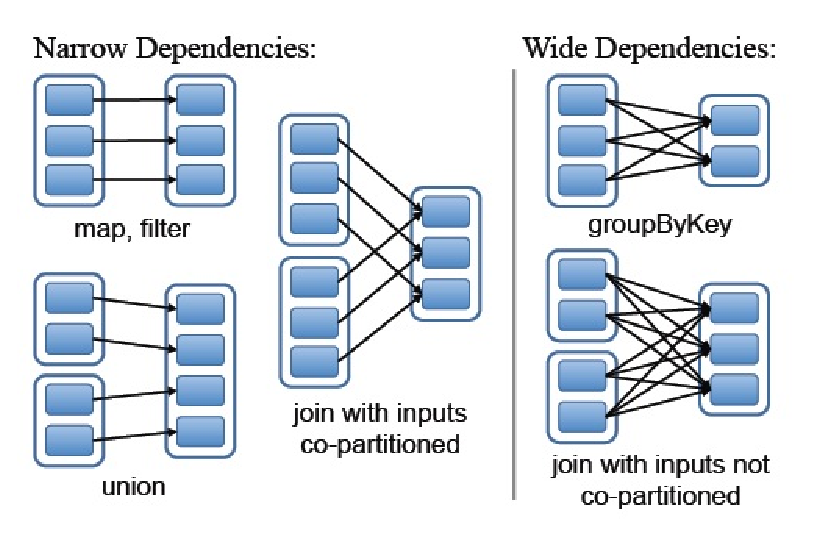
\includegraphics[keepaspectratio=true,scale=0.7]
                            {figuras/figura15.eps}
                        \caption[\textit{Narrow} e \textit{Wide dependencies}. Cada caixa é um RDD com as partições em amostra nos retângulo]
                        {\textit{Narrow} e \textit{Wide dependencies}. Cada caixa é um RDD com as partições em amostra nos retângulo -
                        \protect  Fonte: \citeonline{zaharia2013}}
                        \label{figura15}
            \end{figure}

            Agendar \textit{jobs} no \textit{Spark} é uma tarefa fácil pois na visão do usuário, que é caixa preta, as transformações
            ocorrem de forma paralela, mas internamente o usuário executa uma ação no RDD, o sistema de agendamento examina
            o grafo de \textit{lineage} do RDD para construir um ciclo de estágios a serem executados como é ilustrado na figura
            \ref{figura16}.  Cada estágio contém várias transformações em \textit{pipeline} com \textit{narrow dependencies}. Nas
            fronteiras de cada estágio, ocorre a operação de \textit{shuffle} que são necessárias para as \textit{wide dependencies}.
            O sistema de agentamento então lança as \textit{tasks} para processar as partições restantes de cada estágio até que o
            RDD alvo seja totalmente computado \cite{karau2015}.

            O sistema de agendamento aloca tarefas as maquinas baseado na localidade do dado usando um atraso de agendamento.
            Se uma tarefa precisa de processar uma partição que está disponível em memória em um \textit{node}, a tarefa é enviada
            a aquele \textit{node}. Do contrário, a tarefa processa a partição para o RDD que possui as localizações preferenciais no
            caso do RDD, e envia esse resultado computado ao cliente final que requisitou o processamento \cite{zaharia2013}.

             \begin{figure}[ht!]
                        \centering
                        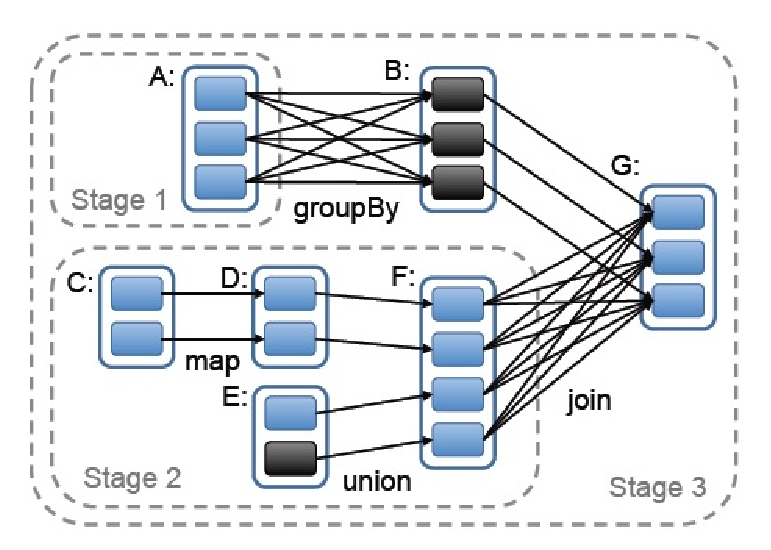
\includegraphics[keepaspectratio=true,scale=0.7]
                            {figuras/figura16.eps}
                        \caption[Estrutura do Spark sobre como ele processa os jobs por estágio]
                        {Estrutura do Spark sobre como ele processa os jobs por estágio -
                        \protect  Fonte: \citeonline{zaharia2013}}
                        \label{figura16}
            \end{figure}

    \section{Impala}



